\subsection{Alimentations et masses électriques}
\label{subsec:alimentation}

Les systèmes de séquenceurs, d'allumage de l'inflammateur et de l'expérience sont fortement isolés les uns des autres,
notamment au niveau de leurs alimentations électriques. Chaque système dispose en effet de son propre circuit d'alimentation,
de ses propres batteries et donc de sa propre masse électrique. Cette séparation assure une meilleure fiabilité et une meilleure
sécurité de l'ensemble (une défaillance ou un court-circuit dans un système n'affecte pas les autres) et permet d'adapter la
capacité des batteries et le dimensionnement de chaque circuit aux besoins réels du système qu'il alimente.\\

\begin{minipage}{0.5\textwidth}
    Les batteries utilisées sont des accumulateurs Li-Ion de \SI{3.7}{\volt} et \SI{2.6}{\ampere\hour} au format 18650, comme celui
    présenté à la figure \ref{fig:batterie_RS}. Ce choix repose sur leur densité énergétique, leur fiabilité et la présence d'un
    circuit de protection intégré contre les surcharges, les décharges profondes et les courts-circuits, indispensable à la
    sécurité des systèmes électroniques embarqués. Au total, 10 de ces batteries sont utilisées, réparties entre chaque système.
\end{minipage}
\hfill
\begin{minipage}{0.4\textwidth}
    \centering
    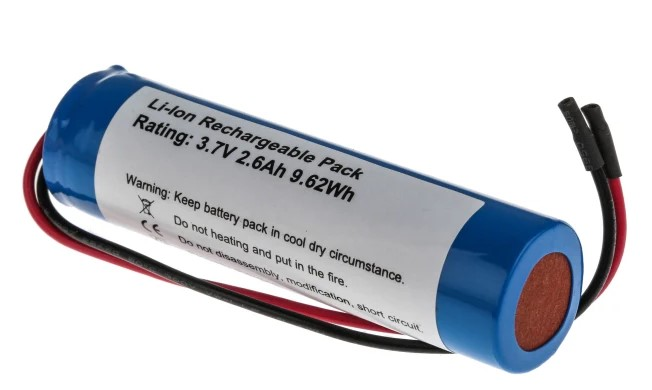
\includegraphics[width=\textwidth]{figures/elec/batterie_RS.jpg}
    \captionof{figure}{Batterie Li-Ion 18650-26H}
    \label{fig:batterie_RS}
\end{minipage}

\vspace{0.2cm}

\subsubsection{Architecture d'alimentation électrique}

La figure \ref{fig:schema_alim} illustre l'architecture d'alimentation électrique des différents systèmes et permet de suivre
le cheminement de l'énergie depuis les batteries jusqu'aux composants électroniques.

\begin{figure}[H]
    \centering
    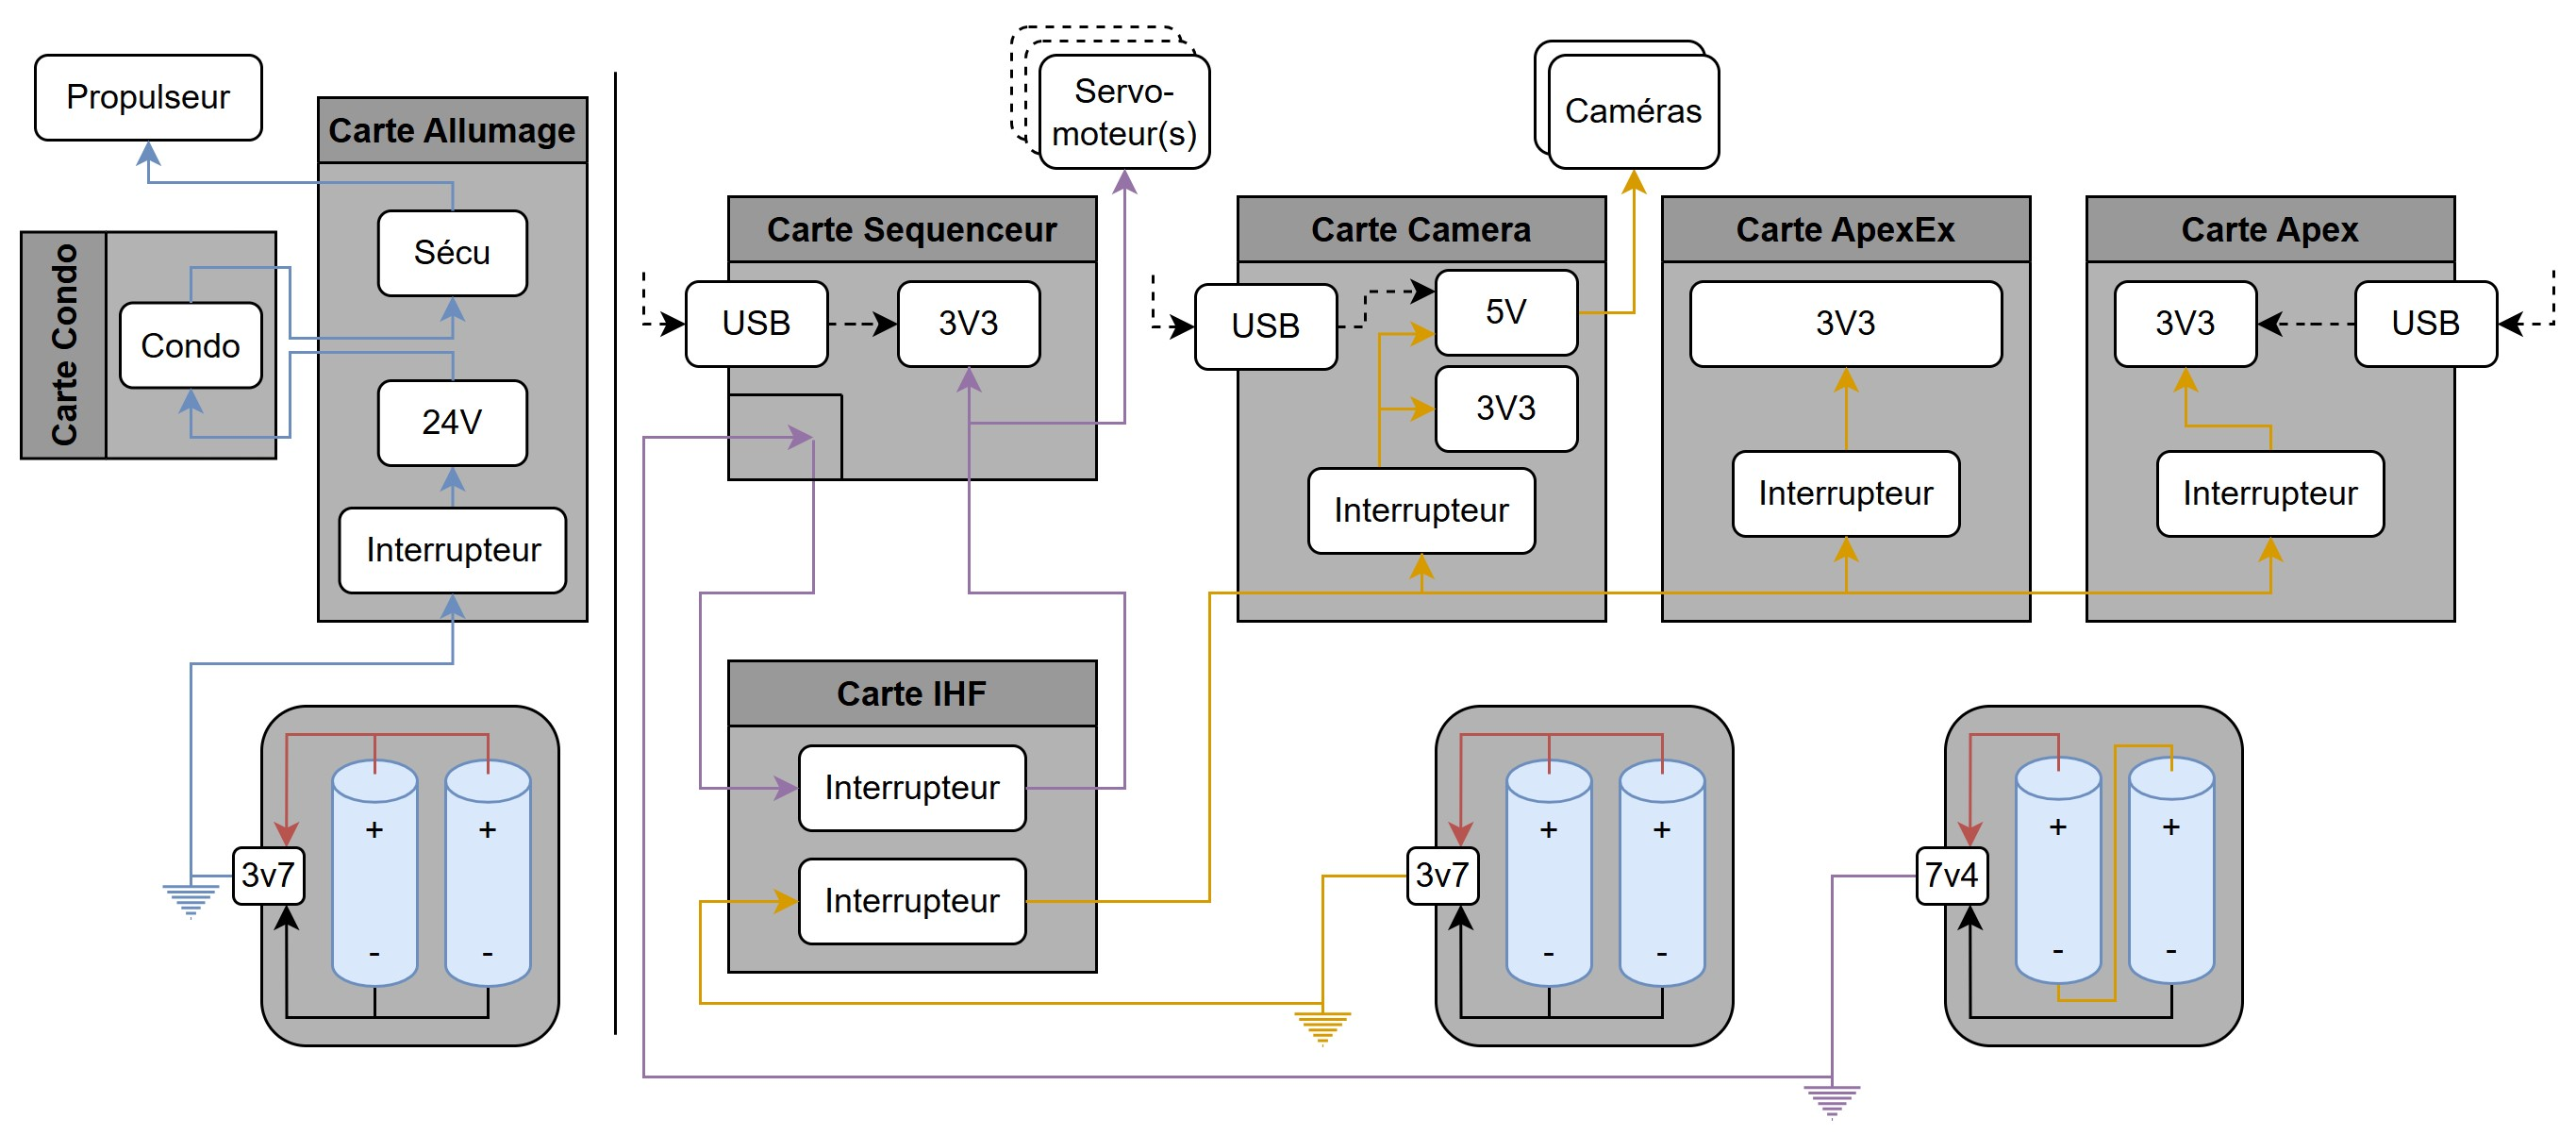
\includegraphics[width=\textwidth]{figures/elec/Schema_alim.jpg}
    \caption{Schéma de l'alimentation électrique des différents systèmes embarqués}
    \label{fig:schema_alim}
\end{figure}

\subsubsubsection{Séquenceur}

Le circuit d'alimentation du séquenceur est représenté en violet sur la figure \ref{fig:schema_alim}. Il est alimenté par un bloc
\verb|1P2S| (deux batteries en série) fournissant une capacité de \SI{2.6}{\ampere\hour} sous une tension nominale de
\SI{7.4}{\volt}. Comme expliqué en sous-section \ref{subsubsubsec:sequenceur_alimentation}, ce bloc est d'abord connecté au
séquenceur, qui redirige la puissance vers l'interrupteur de la carte \acrshort{IHF} avant qu'elle ne revienne sur la carte. Elle y
est alors répartie entre les servomoteurs, alimentés directement sous \SIrange{6.0}{8.0}{\volt}, et un régulateur \SI{3.3}{\volt}
qui alimente l'ensemble des composants logiques.\\

Un port \acrshort{USB} type C permet en outre d'alimenter la partie logique de la carte sans batterie, notamment pour le
développement du logiciel embarqué. Les servomoteurs ne pouvant être alimentés par ce port, la batterie et la carte \acrshort{IHF}
doivent rester connectées au séquenceur pour toute intervention les impliquant.

\newpage

\subsubsubsection{Expérience}

Le circuit d'alimentation de l'expérience est représenté en orange sur la figure \ref{fig:schema_alim}. Il est alimenté par un
bloc \verb|2P1S| (deux batteries en parallèle) fournissant une capacité de \SI{5.2}{\ampere\hour} sous une tension nominale de
\SI{3.7}{\volt}. La puissance transite d'abord par l'interrupteur dédié de la carte \acrshort{IHF}, accessible depuis
l'extérieur de la fusée, puis alimente un bus commun aux trois cartes du système : Apex, ApexEx et Camera.\\

Chacune de ces cartes dispose de son propre interrupteur local, en aval de celui de l'\acrshort{IHF}. Cette double coupure permet
d'isoler individuellement une carte lors des phases d'intégration et d'essais, sans interrompre l'alimentation des autres. La
distribution du bus est réalisée en guirlande (\textit{daisy chain}) : plutôt que de partir d'un point de distribution central, le
bus entre sur une carte, y est dérivé vers l'interrupteur local, puis ressort vers la carte suivante. En aval, chaque carte régule
la tension du bus selon ses besoins : les cartes Apex et ApexEx produisent une unique tension de \SI{3.3}{\volt} destinée à leurs
composants logiques, tandis que la carte Camera génère en plus une tension de \SI{5}{\volt} alimentant les caméras.\\

Comme pour le séquenceur, les cartes Apex et Camera disposent d'un port \acrshort{USB} type C permettant de les alimenter sans
batterie pendant le développement. La carte ApexEx en est dépourvue : ne comportant pas de microcontrôleur, elle ne peut
fonctionner indépendamment de la carte Apex et n'a donc pas d'usage en alimentation isolée. Cependant, il est nécessaire d'utiliser
la batterie pour alimenter la carte ApexEx. Cela implique alors que la carte Apex soit également alimentée par batterie pour que
ces dernières puissent partager une masse commune.

\subsubsubsection{Ligne de mise à feu}

Le circuit de mise à feu est représenté en bleu sur la figure \ref{fig:schema_alim}. Contrairement aux deux circuits
précédents, présents sur les deux étages, celui-ci n'équipe que le second : lui seul embarque un propulseur à allumer en vol.
Il dispose de sa propre batterie et de sa propre masse, et constitue le domaine le plus fortement isolé de l'ensemble.\\

L'énergie provient d'un bloc \verb|2P1S| dédié, de \SI{5.2}{\ampere\hour} sous \SI{3.7}{\volt}. Cette capacité est très
largement supérieure au besoin réel du circuit : la charge des condensateurs pouvant s'effectuer lentement, une batterie de
capacité bien moindre à tension identique aurait suffi. Ce surdimensionnement est délibéré. Une architecture alternative a en
effet été envisagée au cours du développement, dans laquelle l'inflammateur est alimenté directement par la batterie, sans
étage capacitif intermédiaire. Nettement plus simple, cette solution exige en revanche une capacité de décharge instantanée
élevée, donc une batterie de capacité supérieure. La conserver permettait ainsi de basculer vers cette architecture de
secours si le circuit à condensateurs ne s'était pas révélé suffisamment fiable en fin de développement.

\subsubsection{Masses électriques}

L'isolation des alimentations décrite précédemment se traduit directement au niveau des masses : chaque circuit possède sa propre
référence de potentiel, sans liaison avec les autres. La seule exception concerne les deux séquenceurs, qui partagent une masse
commune lorsque les étages sont assemblés.\\

Il en résulte quatre plans de masse distincts sur la fusée assemblée. Celui :
\begin{itemize}
    \item des deux séquenceurs ;
    \item de l'expérience du premier étage ;
    \item de l'expérience du second étage ;
    \item de la ligne de mise à feu.
\end{itemize}
La séparation inter-étage rompt la liaison entre les deux séquenceurs, qui retrouvent alors chacun une masse indépendante. Le
premier étage compte dès lors deux plans de masse (séquenceur et expérience) et le second, trois, la ligne de mise à feu s'ajoutand
aux deux précédents.\\

Le \acrshort{CDC} Fusex bi-étage fait par ailleurs référence à un plan de masse mécanique, auquel les masses électriques doivent
être rapportées. Le projet SP-02 n'en dispose pas : la fusée ne comporte ni treillis porteur ni structure conductrice, sa peau étant
réalisée en fibre de verre. Aucune référence de potentiel n'est donc offerte par la structure, et l'ensemble des masses électriques
reste flottant par rapport à celle-ci.
